\documentclass{article}

\usepackage{alltt}
\usepackage{amsmath}
\usepackage{amssymb}
\usepackage{amsthm}
\usepackage{array}
\usepackage[T1]{fontenc}
\usepackage{geometry}
\usepackage{graphicx}
\usepackage{multicol}
\usepackage{semantic}
\usepackage{tabularx}

\theoremstyle{definition}
\newtheorem{theorem}{Theorem}
\newtheorem{corollary}{Corollary}
\newtheorem{lemma}{Lemma}
\newtheorem{definition}{Definition}

\newcommand{\at}{\ensuremath{{\scriptstyle{@}}}}
\newcommand{\pc}{\ensuremath{{\mathit{pc}}}}

\newcommand{\CoqSymbol}
{\raisebox{-.2ex}{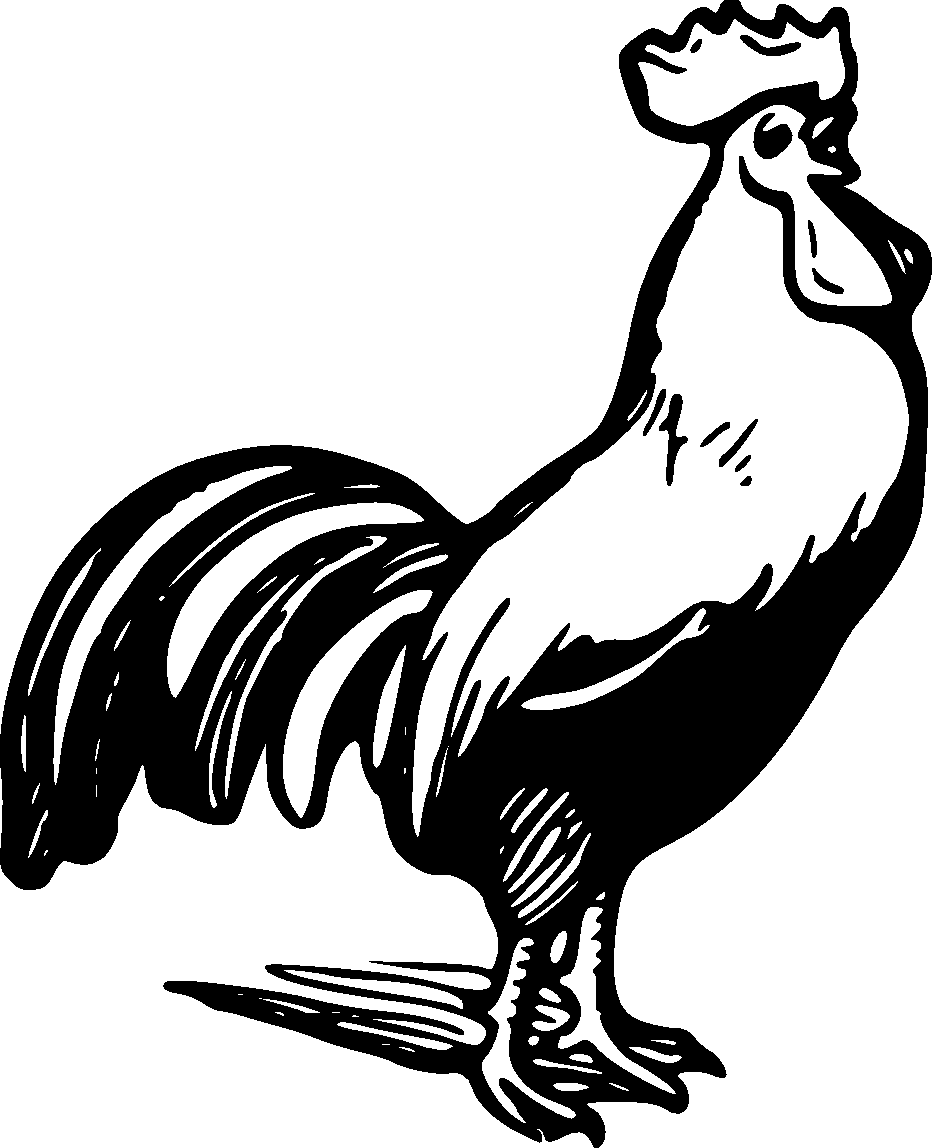
\includegraphics[height=0.9em]{coq.pdf}}\,}
\newcommand{\Coqed}{\hfill\CoqSymbol}

\renewcommand*{\descriptionlabel}[1]{\hspace\labelsep\normalfont #1}

\begin{document}

\begin{flushright}
  \today
\end{flushright}

\begin{figure}[ht]
  \centering
  \[
  \mathcal{L} = \{ \bot, \top \}
  \qquad
  \bot \sqsubseteq \top
  \qquad
  L^{\mathit{def}} = \bot
  \qquad
  \mathcal{A} = \mathbf{1}
  \]
  \[
  \begin{array}[t]{lcl}
    b & ::= &
    \mathit{tt}\;\; |\;\;
    \mathit{ff}
    \\[0.3ex]
    c & :: = &
    b\;\; |\;\;
    n
    \\[0.3ex]
    e & ::= &
    c\;\; |\;\;
    x\;\; |\;\;
    \lambda{x}.\, e\;\; |\;\;
    e\ e\;\; |\;\;
    \mathsf{declassify}\ e\ e
    \\[0.3ex]
    v & ::= &
    c\;\; |\;\;
    \langle{\lambda{x}.\, e, \rho\rangle}
    \\[0.3ex]
    a & ::= &
    v \at L
    \\[0.3ex]
    \rho & ::= &
    \bullet\;\; |\;\;
    \rho[x = a]
  \end{array}
  \]
  \caption{Syntax of $\lambda_{\mathbf{2}}$.}
  \label{fig:syntax}
\end{figure}

\begin{definition}
  The $\approx^{L}_{P}$ relation expresses the \emph{indistinguishability} of
  atoms for observers at label $L$, with respect to some reflexive relation
  on values $P$, where $v_1 \at L_1 \approx^{L}_{P} v_2 \at L_2$ iff either
  \begin{itemize}
  \item
    $L = \bot$ and
    $L_1 = L_2 = \top$ and either
    \begin{itemize}
    \item
      $v_1 = n_1$ and
      $v_2 = n_2$ and
      $P(v_1, v_2)$, or
    \item
      $v_1 = \langle{\lambda{x_1}.\, e_1, \rho_1\rangle}$ and
      $v_2 = \langle{\lambda{x_2}.\, e_2, \rho_2\rangle}$ and
      $v_1 \approx^{L}_{P} v_2$, or
    \item
      $v_1 = c_1$ and $v_2 = \langle{\lambda{x_2}.\, e_2, \rho_2\rangle}$, or
    \item
      $v_1 = \langle{\lambda{x_1}.\, e_1, \rho_1\rangle}$ and $v_2 = c_2$; or
    \end{itemize}
  \item $L = \bot$ and
    $L_1 = L_2 = \bot$ and $v_1 \approx^{L}_{P} v_2$; or
  \item $L = \top$ and $L_1 = L_2$ and $v_1 \approx^{L}_{P} v_2$.
  \end{itemize}
  The definition for atoms is mutually recursive with that for values and
  environments:
  \begin{itemize}
  \item $c_1 \approx^{L}_{P} c_2$ iff $c_1 = c_2$.
  \item
    $\langle{\lambda{x_1}.\, e_1, \rho_1\rangle} \approx^{L}_{P}
    \langle{\lambda{x_2}.\, e_2, \rho_2\rangle}$ iff
    $\lambda{x_1}.\, e_1 \equiv \lambda{x_2}.\, e_2$ and
    $\rho_1 \approx^{L}_{P} \rho_2$.
  \item $\rho_1 \approx^{L}_{P} \rho_2$ iff
    $\mathrm{dom}\; \rho_1 = \mathrm{dom}\; \rho_2$ and
    $\rho_1(x) \approx^{L}_{P} \rho_2(x)$ for every
    $x \in \mathrm{dom}\; \rho_1$.
  \end{itemize}
  We write $\approx^{L}$ when $P$ is the everywhere-true relation.
  \label{def:lp-equiv}
\end{definition}

\begin{lemma}
  $\approx^{L}_{P}$ implies $\approx^{L}$.
  \begin{enumerate}
  \item If $a_1 \approx^{L}_{P} a_2$, then $a_1 \approx^{L} a_2$.
  \item If $v_1 \approx^{L}_{P} v_2$, then $v_1 \approx^{L} v_2$.
  \item If $\rho_1 \approx^{L}_{P} \rho_2$, then $\rho_1 \approx^{L} \rho_2$.
  \Coqed
  \end{enumerate}
  \label{lem:lp-equiv-l-equiv}
\end{lemma}

\begin{lemma}
  $\approx^{L}_{P}$ is reflexive.
  \Coqed
  \label{lem:lp-equiv-refl}
\end{lemma}

% \begin{lemma}
%  If $v_1 \at L_1 \approx^{L}_{P} v_2 \at L_2$, then $L_1 = L_2$.
%  \Coqed
%  \label{lem:lp-equiv-lab-inv}
% \end{lemma}

\begin{lemma}
  If $v_1 \at \bot \approx^{L}_{P} v_2 \at \bot$, then
  $v_1 \at \top \approx^{L}_{P} v_2 \at \top$.
  \Coqed
  \label{lem:lp-equiv-raise}
\end{lemma}

\pagebreak

\begin{figure}[ht]
  \centering
  \begin{gather*}
    \inference{}{
      \langle{L, P, \pc, \rho\rangle} |-
      c
      \Downarrow^{k}_{l}
      c \at \pc
    }[\textsc{E-Const}]
    \qquad
    \inference{
      {\begin{array}{l}
          \rho(x) = v \at L_1
        \end{array}}
    }{
      \langle{P, L, \pc, \rho\rangle} |-
      x
      \Downarrow^{k}_{l}
      v \at (\pc \sqcup L_1)
    }[\textsc{E-Var}]
    \\[3ex]
    \inference{}{
      \langle{L, P, \pc, \rho\rangle} |-
      (\lambda{x}.\, e)
      \Downarrow^{k}_{l}
      \langle{\lambda{x}.\, e, \rho\rangle} \at \pc
    }[\textsc{E-Abs}]
    \qquad
    \inference{
      {\begin{array}{l}
          \langle{L, P, \pc, \rho\rangle} |-
          e_1
          \Downarrow^{k}_{l}
          \langle{\lambda{x}.\, e, \rho_1\rangle} \at L_1
          \\
          \langle{L, P, \pc, \rho\rangle} |-
          e_2 \Downarrow^{k}_{l} a_2
          \\
          \langle{L, P, L_1, \rho_1[x = a_2]\rangle} |-
          e
          \Downarrow^{k}_{l}
          a_3
        \end{array}}
    }{
      \langle{L, P, \pc, \rho\rangle} |-
      (e_1\ e_2)
      \Downarrow^{k+1}_{l}
      a_3
    }[\textsc{E-App}]
    \\[3ex]
    \inference{
      {\begin{array}{l}
          \langle{L, P, \pc, \rho\rangle} |-
          (e_1\ e_2)
          \Downarrow^{k}_{l}
          v \at \bot
        \end{array}}
    }{
      \langle{L, P, \pc, \rho\rangle} |-
      (\mathsf{declassify}\ e_1\ e_2)
      \Downarrow^{k+1}_{l}
      v \at \bot
    }[\textsc{E-Decl1}]
    \\[3ex]
    \inference{
      {\begin{array}{l}
          \langle{L, P, \pc, \rho\rangle} |-
          e_1
          \Downarrow^{k}_{l}
          \langle{\lambda{x}.\, e, \rho_1\rangle} \at L_1
          \\
          \langle{L, P, \pc, \rho\rangle} |-
          e_2
          \Downarrow^{k}_{l}
          a_2
          \\
          \langle{L, P, L_1, \rho_1[x = a_2]\rangle} |-
          e
          \Downarrow^{k}_{l}
          v_3 \at \top
          \\
          \forall{\rho_1', a_2' \text{ s.t. }
            \rho_1[x = a_2] \approx^{L}_{P} \rho_1'[x = a_2']}.
          \\\quad
          \langle{L, P, L_1, \rho_1'[x = a_2']\rangle} |-
          e
          \Downarrow^{l}_{k}
          v_3' \at \top =>
          v_3 \approx^{L}_{P} v_3'
        \end{array}}
    }{
      \langle{L, P, \pc, \rho\rangle} |-
      (\mathsf{declassify}\ e_1\ e_2)
      \Downarrow^{k+1}_{l}
      v_3 \at \bot
    }[\textsc{E-Decl2}]
    \\[3ex]
    \langle{L, P, \pc, \rho\rangle} |-
    e
    \Downarrow
    a
    \quad \triangleq \quad
    \exists{k}.\, \forall{l}.\,
    \langle{L, P, \pc, \rho\rangle} |-
    e
    \Downarrow^{k}_{l}
    a
  \end{gather*}
  \caption{Semantics of $\lambda_{\mathbf{2}}$.}
  \label{fig:semantics}
\end{figure}

\begin{lemma}
  $\Downarrow^{k}_{l}\ \subseteq\ \Downarrow^{k+1}_{l}$
  and
  $\Downarrow^{k}_{l+1}\ \subseteq\ \Downarrow^{k}_{l}$.
  \label{lem:semantics-step-subset}
\end{lemma}
\begin{proof}
  It suffices to show that for all $k$ and $l$ such that $k + l < n$, for
  any $n$:
  \begin{flalign}
    & \quad
    \text{If $\langle{L, P, \pc, \rho\rangle} |- e \Downarrow^{k}_{l} a$, then
      $\langle{L, P, \pc, \rho\rangle} |- \Downarrow^{k+1}_{l} a$.}
    \label{ih:semantics-step-subset-k-k+1} & \\
    & \quad
    \text{If $\langle{L, P, \pc, \rho\rangle} |- e \Downarrow^{k}_{l+1} a$, then
      $\langle{L, P, \pc, \rho\rangle} |- e \Downarrow^{k}_{l} a$.}
    \label{ih:semantics-step-subset-l+1-l} &
  \end{flalign}
  The proof is by induction on $n$. Note that the claim is vacuously true
  when $n = 0$. Assume the claim holds for all $k$ and $l$ such that
  $k + l < n$ for some $n$. We must show that it is true for all
  $k + l < n + 1$, that is, when $k + l = n$. We proceed by case analysis
  on the structure of $e$.

  The cases for constants $c$, variables $x$, and abstractions
  $(\lambda{x}.\, e)$ are immediate, while the case for applications
  $(e_1\ e_2)$ follows from a simple application of the induction hypothesis.
  We consider the final case for declassification operations
  $(\mathsf{declassify}\ e_1\ e_2)$ below.
  \begin{enumerate}
  \item By inversion, $k > 0$ and the derivation is by:
    \begin{itemize}
    \item \textsc{E-Decl1}, in which case
      $\langle{L, P, \pc, \rho\rangle} |- (\mathsf{declassify}\ e_1\ e_2)
      \Downarrow^{k}_{l} v \at \bot$ and by inversion
      $\langle{L, P, \pc, \rho\rangle} |- (e_1\ e_2) \Downarrow^{k-1}_{l}
      v \at \bot$. Since $k-1 + l < n$, we can apply the induction
      hypothesis~(\ref{ih:semantics-step-subset-k-k+1}) to get
      $\langle{L, P, \pc, \rho\rangle} |- (e_1\ e_2) \Downarrow^{k}_{l}
      v \at \bot$. By \textsc{E-Decl1}, we have
      \[\langle{L, P, \pc, \rho\rangle} |- (\mathsf{declassify}\ e_1\ e_2)
      \Downarrow^{k+1}_{l} v \at \bot.\]
    \item \textsc{E-Decl2}, in which case
      $\langle{L, P, \pc, \rho\rangle} |- (\mathsf{declassify}\ e_1\ e_2)
      \Downarrow^{k}_{l} v_3 \at \bot$ and by inversion:
      \begin{center}
        \begin{tabular*}{1.0\linewidth}{ll}
          a.
          $\langle{L, P, \pc, \rho\rangle} |- e_1
          \Downarrow^{k-1}_{l}
          \langle{\lambda{x}.\, e, \rho_1\rangle} \at L_1$
          &
          b.
          $\langle{L, P, \pc, \rho\rangle} |- e_2
          \Downarrow^{k-1}_{l}
          a_2$
          \\[1.8ex]
          c.
          $\langle{L, P, L_1, \rho_1[x = a_2]\rangle} |- e
          \Downarrow^{k-1}_{l}
          v_3 \at \top$
          &
          d.
          $\forall{\rho_1', a_2' \text{ s.t. }
            \rho_1[x = a_2] \approx^{L}_{P} \rho_1'[x = a_2']}.$
          \\
          &
          \quad\quad
          $\langle{L, P, L_1, \rho_1'[x = a_2']\rangle} |- e
          \Downarrow^{l}_{k-1} v_3' \at \top$
          \\
          &
          \quad\quad
          $=>
          v_3 \approx^{L}_{P} v_3'$
        \end{tabular*}
      \end{center}
      Since $k-1 + l < n$, we can apply the induction
      hypothesis~(\ref{ih:semantics-step-subset-k-k+1}) to a, b, and c,
      getting a', b', and c'; and since
      $\Downarrow^{l}_{k}\ \subseteq\ \Downarrow^{l}_{k-1}$ by
      the induction hypothesis~(\ref{ih:semantics-step-subset-l+1-l}),
      we also get d':
      \begin{center}
        \begin{tabular*}{1.0\linewidth}{l@{\qquad}l}
          a'.
          $\langle{L, P, \pc, \rho\rangle} |- e_1
          \Downarrow^{k}_{l}
          \langle{\lambda{x}.\, e, \rho_1\rangle} \at L_1$
          &
          b'.
          $\langle{L, P, \pc, \rho\rangle} |- e_2
          \Downarrow^{k}_{l}
          a_2$
          \\[1.8ex]
          c'.
          $\langle{L, P, L_1, \rho_1[x = a_2]\rangle} |- e
          \Downarrow^{k}_{l}
          v_3 \at \top$
          &
          d'.
          $\forall{\rho_1', a_2' \text{ s.t. }
            \rho_1[x = a_2] \approx^{L}_{P} \rho_1'[x = a_2']}.$
          \\
          &
          \quad\quad
          $\langle{L, P, L_1, \rho_1'[x = a_2']\rangle} |- e
          \Downarrow^{l}_{k} v_3' \at \top$
          \\
          &
          \quad\quad
          $=>
          v_3 \approx^{L}_{P} v_3'$
        \end{tabular*}
      \end{center}
      By \textsc{E-Decl2}, we have
      $\langle{L, P, \pc, \rho\rangle} |- (\mathsf{declassify}\ e_1\ e_2)
      \Downarrow^{k+1}_{l}
      v_3 \at \bot$.
    \end{itemize}
  \item By inversion, $k > 0$ and the derivation is by:
    \begin{itemize}
    \item \textsc{E-Decl1}, in which case
      $\langle{L, P, \pc, \rho\rangle} |- (\mathsf{declassify}\ e_1\ e_2)
      \Downarrow^{k}_{l+1}
      v \at \bot$ and by inversion
      $\langle{L, P, \pc, \rho\rangle} |- (e_1\ e_2)
      \Downarrow^{k-1}_{l+1} v \at \bot$.
      Since $k-1 + l < n$, we can apply the induction
      hypothesis~(\ref{ih:semantics-step-subset-l+1-l}) to get
      $\langle{L, P, \pc, \rho\rangle} |- (e_1\ e_2)
      \Downarrow^{k-1}_{l} v \at \bot$.
      By \textsc{E-Decl1}, we have
      \[ \langle{L, P, \pc, \rho\rangle} |- (e_1\ e_2)
      \Downarrow^{k}_{l} v \at \bot. \]
    \item \textsc{E-Decl2}, in which case
      $\langle{L, P, \pc, \rho\rangle} |- (\mathsf{declassify}\ e_1\ e_2)
      \Downarrow^{k}_{l+1}
      v_3 \at \bot$ and by inversion:
      \begin{center}
        \begin{tabular*}{1.0\linewidth}{ll}
          a.
          $\langle{L, P, \pc, \rho\rangle} |- e_1
          \Downarrow^{k-1}_{l+1}
          \langle{\lambda{x}.\, e, \rho_1\rangle} \at L_1$
          &
          b.
          $\langle{L, P, \pc, \rho\rangle} |- e_2
          \Downarrow^{k-1}_{l+1}
          a_2$
          \\[1.8ex]
          c.
          $\langle{L, P, L_1, \rho_1[x = a_2]\rangle} |- e
          \Downarrow^{k-1}_{l+1}
          v_3 \at \top$
          &
          d.
          $\forall{\rho_1', a_2' \text{ s.t. }
            \rho_1[x = a_2] \approx^{L}_{P} \rho_1'[x = a_2']}.$
          \\ & \quad\quad
          $\langle{L, P, L_1, \rho_1'[x = a_2']\rangle} |- e
          \Downarrow^{l+1}_{k-1} v_3' \at \top$
          \\ & \quad\quad
          $=> v_3 \approx^{L}_{P} v_3'$
        \end{tabular*}
      \end{center}
      Since $k-1 + l < n$, we can apply the induction
      hypothesis~(\ref{ih:semantics-step-subset-l+1-l}) to a, b, and c,
      getting a', b', and c'; and since
      $\Downarrow^{l}_{k-1}\ \subseteq\ \Downarrow^{l+1}_{k-1}$
      by the induction hypothesis~(\ref{ih:semantics-step-subset-k-k+1}),
      we also get d':
      \begin{center}
        \begin{tabular*}{1.0\linewidth}{ll}
          a'.
          $\langle{L, P, \pc, \rho\rangle} |- e_1
          \Downarrow^{k-1}_{l}
          \langle{\lambda{x}.\, e, \rho_1\rangle} \at L_1$
          &
          b'.
          $\langle{L, P, \pc, \rho\rangle} |- e_2
          \Downarrow^{k-1}_{l}
          a_2$
          \\[1.8ex]
          c'.
          $\langle{L, P, L_1, \rho_1[x = a_2]\rangle} |- e
          \Downarrow^{k-1}_{l}
          v_3 \at \top$
          &
          d'.
          $\forall{\rho_1', a_2' \text{ s.t. }
            \rho_1[x = a_2] \approx^{L}_{P} \rho_1'[x = a_2']}.$
          \\ & \quad\quad
          $\langle{L, P, L_1, \rho_1'[x = a_2']\rangle} |- e
          \Downarrow^{l}_{k-1} v_3' \at \top$
          \\ & \quad\quad
          $=> v_3 \approx^{L}_{P} v_3'$
        \end{tabular*}
      \end{center}
      By \textsc{E-Decl2}, we have
      $\langle{L, P, \pc, \rho\rangle} |- (\mathsf{declassify}\ e_1\ e_2)
      \Downarrow^{k}_{l}
      v_3 \at \bot$.
      \qedhere
    \end{itemize}
  \end{enumerate}
\end{proof}

\pagebreak

\begin{theorem}
  If $\langle{L, P, \pc, \rho\rangle} |- e \Downarrow a$ and
  $\langle{L, P, \pc, \rho'\rangle} |- e \Downarrow a'$ and
  $\rho \approx^{L}_{P} \rho'$, then $a \approx^{L}_{P} a'$.
  \label{thm:non-interference}
\end{theorem}
\begin{proof}
  Unfolding the definition of $\Downarrow$, the claim is:
  \begin{flalign*}
    & \quad
    \text{If $\exists{k}.\, \forall{l}.\,
      \langle{L, P, \pc, \rho\rangle} |- e \Downarrow^{k}_{l} a$ and
      $\exists{k'}.\, \forall{l}.\,
      \langle{L, P, \pc, \rho'\rangle} |- e \Downarrow^{k'}_{l} a'$ and
      $\rho \approx^{L}_{P} a'$, then $a \approx^{L}_{P} a'$.}
    &
  \end{flalign*}
  It suffices to show that for all $k$ and $k'$ such that $k + k' < n$, for
  any $n$:
  \begin{flalign}
    & \quad
    \text{If $\forall{l}.\,
      \langle{L, P, \pc, \rho\rangle} |- e \Downarrow^{k}_{l} a$ and
      $\forall{l}.\,
      \langle{L, P, \pc, \rho'\rangle} |- e \Downarrow^{k'}_{l} a'$ and
      $\rho \approx^{L}_{P} a'$, then $a \approx^{L}_{P} a'$.}
    \label{ih:non-interference} &
  \end{flalign}
  The proof is by induction on $n$. Note that the claim is vacuously true when
  $n = 0$. Assume the claim holds for some $n$ such that $k + k' < n$.
  We must show that it is true for $k + k' < n + 1$, that is, when
  $k + k' = n$. We proceed by case analysis on the structure of $e$.

  The cases for constants $c$, variables $x$, and abstractions
  $(\lambda{x}.\, e)$ are straightforward, while the cases for applications
  $(e_1\ e_2)$ and declassification operations
  $(\mathsf{declassify}\ e_1\ e_2)$, when the derivations are by
  \textsc{E-Decl1}, follow from a simple application of the induction
  hypothesis.

  For the final case of declassification operations when the derivations
  are by \textsc{E-Decl2}, we have, by inversion of the derivations of $a$
  and $a'$, that $k > 0$ and $k' > 0$ and, for all $l$:
  \begin{gather*}
    \inference{
      {\begin{array}{l}
          \langle{L, P, \pc, \rho\rangle} |-
          e_1
          \Downarrow^{k-1}_{l}
          \langle{\lambda{x}.\, e, \rho_1\rangle} \at L_1
          \\
          \langle{L, P, \pc, \rho\rangle} |-
          e_2
          \Downarrow^{k-1}_{l}
          a_2
          \\
          \langle{L, P, L_1, \rho_1[x = a_2]\rangle} |-
          e
          \Downarrow^{k-1}_{l}
          v_3 \at \top
          \\
          \forall{\rho_1', a_2' \text{ s.t. }
            \rho_1[x = a_2] \approx^{L}_{P} \rho_1'[x = a_2']}.
          \\\quad
          \langle{L, P, L_1, \rho_1'[x = a_2']\rangle} |-
          e
          \Downarrow^{l}_{k-1}
          v_3' \at \top
          \\\quad =>
          v_3 \approx^{L}_{P} v_3'
        \end{array}}
    }{
      \langle{L, P, \pc, \rho\rangle} |-
      (\mathsf{declassify}\ e_1\ e_2)
      \Downarrow^{k}_{l}
      v_3 \at \bot
    }
    \quad
    \inference{
      {\begin{array}{l}
          \langle{L, P, \pc, \rho'\rangle} |-
          e_1
          \Downarrow^{k'-1}_{l}
          \langle{\lambda{x}.\, e', \rho_1'\rangle} \at L_1'
          \\
          \langle{L, P, \pc, \rho'\rangle} |-
          e_2
          \Downarrow^{k'-1}_{l}
          a_2'
          \\
          \langle{L, P, L_1', \rho_1'[x = a_2']\rangle} |-
          e'
          \Downarrow^{k'-1}_{l}
          v_3' \at \top
          \\
          \forall{\rho_1'', a_2'' \text{ s.t. }
            \rho_1'[x = a_2'] \approx^{L}_{P} \rho_1''[x = a_2'']}.
          \\\quad
          \langle{L, P, L_1', \rho_1''[x = a_2'']\rangle} |-
          e'
          \Downarrow^{l}_{k'-1}
          v_3'' \at \top
          \\\quad =>
          v_3' \approx^{L}_{P} v_3''
        \end{array}}
    }{
      \langle{L, P, \pc, \rho'\rangle} |-
      (\mathsf{declassify}\ e_1\ e_2)
      \Downarrow^{k'}_{l}
      v_3' \at \bot
    }
  \end{gather*}

  Since $(k-1) + (k'-1) < n$, we can apply the induction
  hypothesis~(\ref{ih:non-interference})
  to the first three pairs of premises.
  First, we get
  $\langle{\lambda{x}.\, e, \rho_1\rangle} \at L_1
  \approx^{L}_{P}
  \langle{\lambda{x}.\, e', \rho_1'\rangle} \at L_1'$.
  It follows by inversion of the $\approx^{L}_{P}$ relation that
  $e = e'$, $L_1 = L_1'$, and $\rho_1 \approx^{L}_{P} \rho_1'$.
  Second, we get $a_2 \approx^{L}_{P} a_2'$.
  Since $\rho_1 \approx^{L}_{P} \rho_1'$, it follows that
  $\rho_1[x = a_2] \approx^{L}_{P} \rho_1'[x = a_2']$.
  Finally we get $v_3 \at \top \approx^{L}_{P} v_3' \at \top$,
  and must show that $v_3 \at \bot \approx^{L}_{P} v_3' \at \bot$.

  Consider the fourth premise.
  We already have $\rho_1[x = a_2] \approx^{L}_{P} \rho_1'[x = a_2']$ and,
  for all $l$, that
  $\langle{L, P, L_1, \rho_1'[x = a_2']\rangle} |- e
  \Downarrow^{k'-1}_{l} v_3' \at \top$.
  Without loss of generality, we can assume $k \leq l$ and $k' \leq l$.
  By Lemma~\ref{lem:semantics-step-subset}, it follows that
  $\Downarrow^{k'-1}_{l}\ \subseteq\ \Downarrow^{l}_{k-1}$ and therefore
  $\langle{L, P, L_1, \rho_1'[x = a_2']\rangle} |- e \Downarrow^{l}_{k-1}
  v_3' \at \top$. Applying fourth premise, we get $v_3 \approx^{L}_{P} v_3'$
  and therefore $v_3 \at \bot \approx^{L}_{P} v_3' \at \bot$.
  % \begin{description}
  % \item[\emph{Case} $c$:]
  %   \begin{gather*}
  %     \inference{}{
  %       \langle{L, P, \pc, \rho\rangle} |- c \Downarrow^{k}_{l} c \at \pc
  %     }
  %     \quad
  %     \inference{}{
  %       \langle{L, P, \pc, \rho'\rangle} |- c \Downarrow^{k'}_{l} c \at \pc
  %     }
  %   \end{gather*}
  %   By Lemma~\ref{lem:lp-equiv-refl}, we have
  %   $c \at \pc \approx^{L}_{P} c \at \pc$.
  % \item[\emph{Case} $x$:]
  %   \begin{gather*}
  %     \inference{
  %       \rho(x) = v \at L_1
  %     }{
  %       \langle{L, P, \pc, \rho\rangle} |-
  %       x
  %       \Downarrow^{k}_{l}
  %       v \at (\pc \sqcup L_1)
  %     }
  %     \quad
  %     \inference{
  %       \rho'(x) = v' \at L_1'
  %     }{
  %       \langle{L, P, \pc, \rho'\rangle} |-
  %       x
  %       \Downarrow^{k'}_{l}
  %       v' \at (\pc \sqcup L_1')
  %     }
  %   \end{gather*}
  %   Since $\rho \approx^{L}_{P} \rho'$, we have
  %   $v \at L_1 \approx v' \at L_1'$.
  %   By inversion, $L_1 = L_1'$. Therefore we must show
  %   that $v \at (\pc \sqcup L_1) \approx^{L}_{P} v' \at (\pc \sqcup L_1)$.
  %   We proceed by case analysis on $\pc$ and $L_1$.
  %   % 
  %   If $pc = \bot$, or if $\pc = \top$ and $L_1 = \top$, then
  %   $\pc \sqcup L_1 = L_1$ and we have
  %   $v \at (\pc \sqcup L_1) \approx^{L}_{P} v' \at (\pc \sqcup L_1)$
  %   immediately.
  %   %
  %   If $pc = \top$ and $L_1 = \bot$, then $\pc \sqcup L_1 = \pc$ and,
  %   by Lemma~\ref{lem:lp-equiv-raise},
  %   $v \at (\pc \sqcup L_1) \approx^{L}_{P} v' \at (\pc \sqcup L_1)$.
  % \item[\emph{Case} $(\lambda{x}.\, e)$:]
  %   \begin{gather*}
  %     \inference{}{
  %       \langle{L, P, \pc, \rho\rangle} |-
  %       (\lambda{x}.\, e)
  %       \Downarrow^{k}_{l}
  %       \langle{\lambda{x}.\, e, \rho\rangle} \at \pc
  %     }
  %     \quad
  %     \inference{}{
  %       \langle{L, P, \pc, \rho'\rangle} |-
  %       (\lambda{x}.\, e)
  %       \Downarrow^{k'}_{l}
  %       \langle{\lambda{x}.\, e, \rho'\rangle} \at \pc
  %     }
  %   \end{gather*}
  %   By the definition of $\approx^{L}_{P}$,
  %   $\langle{\lambda{x}.\, e, \rho\rangle} \at \pc
  %   \approx^{L}_{P}
  %   \langle{\lambda{x}.\, e, \rho'\rangle} \at \pc$
  %   iff
  %   $\langle{\lambda{x}.\, e, \rho\rangle}
  %   \approx^{L}_{P}
  %   \langle{\lambda{x}.\, e, \rho'\rangle}$,
  %   which we have immediately, since $\rho \approx^{L}_{P} \rho'$.
  % \item[\emph{Note}:]
  %   For the remaining cases, we have $k > 0$ and $k' > 0$.
  % \item[\emph{Case} $(e_1\ e_2)$:]
  %   \begin{gather*}
  %     \inference{
  %       {\begin{array}{l}
  %           \langle{L, P, \pc, \rho\rangle} |-
  %           e_1
  %           \Downarrow^{k-1}_{l}
  %           \langle{\lambda{x}.\, e, \rho_1\rangle} \at L_1
  %           \\
  %           \langle{L, P, \pc, \rho\rangle} |-
  %           e_2
  %           \Downarrow^{k-1}_{l}
  %           a_2
  %           \\
  %           \langle{L, P, L_1, \rho_1[x = a_2]\rangle} |-
  %           e
  %           \Downarrow^{k-1}_{l}
  %           a_3
  %         \end{array}}
  %     }{
  %       \langle{L, P, \pc, \rho\rangle} |-
  %       (e_1\ e_2)
  %       \Downarrow^{k}_{l}
  %       a_3
  %     }
  %     \quad
  %     \inference{
  %       {\begin{array}{l}
  %           \langle{L, P, \pc, \rho'\rangle} |-
  %           e_1
  %           \Downarrow^{k'-1}_{l}
  %           \langle{\lambda{x}.\, e', \rho_1'\rangle} \at L_1'
  %           \\
  %           \langle{L, P, \pc, \rho'\rangle} |-
  %           e_2
  %           \Downarrow^{k'-1}_{l}
  %           a_2'
  %           \\
  %           \langle{L, P, L_1', \rho_1'[x = a_2']\rangle} |-
  %           e'
  %           \Downarrow^{k'-1}_{l}
  %           a_3'
  %         \end{array}}
  %     }{
  %       \langle{L, P, \pc, \rho'\rangle} |-
  %       (e_1\ e_2)
  %       \Downarrow^{k'}_{l}
  %       a_3'
  %     }
  %   \end{gather*}
  %   Since $(k-1) + (k'-1) < n$, we can apply the induction hypothesis
  %   to each pair of premises:
  %   First,
  %   $\langle{\rho_1, \lambda{x}.\, e\rangle} \at L_1
  %   \approx^{L}_{P}
  %   \langle{\rho_1', \lambda{x}.\, e'\rangle} \at L_1'$,
  %   which means $\rho_1 \approx^{L}_{P} \rho_1'$ and, by inversion,
  %   $e = e'$, and $L_1 = L_1'$.
  %   Second,
  %   $a_2 \approx^{L}_{P} a_2'$,
  %   which means
  %   $(\rho_1, x = a_2) \approx^{L}_{P} (\rho_1', x = a_2')$.
  %   Finally,
  %   $a_3 \approx^{L}_{P} a_3'$,
  %   which completes the case.
  % \item[\emph{Case} $(\mathsf{declassify}\ e_1\ e_2)$:]\
  %   \begin{description}
  %   \item[\emph{Subcase} \textsc{E-Decl1}:]
  %     \begin{gather*}
  %       \inference{
  %         \langle{L, P, \pc, \rho\rangle} |-
  %         (e_1\ e_2)
  %         \Downarrow^{k-1}_{l}
  %         v \at \bot
  %       }{
  %         \langle{L, P, \pc, \rho\rangle} |-
  %         (\mathsf{declassify}\ e_1\ e_2)
  %         \Downarrow^{k-1}_{l}
  %         v \at \bot
  %       }
  %       \\[2ex]
  %       \inference{
  %         \langle{L, P, \pc, \rho'\rangle} |-
  %         (e_1\ e_2)
  %         \Downarrow^{k'-1}_{l}
  %         v' \at \bot
  %       }{
  %         \langle{L, P, \pc, \rho'\rangle} |-
  %         (\mathsf{declassify}\ e_1\ e_2)
  %         \Downarrow^{k'-1}_{l}
  %         v' \at \bot
  %       }
  %     \end{gather*}
  %     Since $(k-1) + (k'-1) < n$, we can apply the induction hypothesis to
  %     the pair of premises, which gives
  %     $v \at \bot \approx^{L}_{P} v' \at \bot$, completing the subcase.
  %   \item[\emph{Subcase} \textsc{E-Decl2}:]
  %     \begin{gather*}
  %       \inference{
  %         {\begin{array}{l}
  %             \langle{L, P, \pc, \rho\rangle} |-
  %             e_1
  %             \Downarrow^{k-1}_{l}
  %             \langle{\lambda{x}.\, e, \rho_1\rangle} \at L_1
  %             \\
  %             \langle{L, P, \pc, \rho\rangle} |-
  %             e_2
  %             \Downarrow^{k-1}_{l}
  %             a_2
  %             \\
  %             \langle{L, P, L_1, \rho_1[x = a_2]\rangle} |-
  %             e
  %             \Downarrow^{k-1}_{l}
  %             v_3 \at \top
  %             \\
  %             \forall{\rho_1', a_2' \text{ s.t. }
  %               \rho_1[x = a_2] \approx^{L}_{P} \rho_1'[x = a_2']}.
  %             \\\quad
  %             \langle{L, P, L_1, \rho_1'[x = a_2']\rangle} |-
  %             e
  %             \Downarrow^{l}_{k-1}
  %             v_3' \at \top =>
  %             v_3 \approx^{L}_{P} v_3'
  %           \end{array}}
  %       }{
  %         \langle{L, P, \pc, \rho\rangle} |-
  %         (\mathsf{declassify}\ e_1\ e_2)
  %         \Downarrow^{k}_{l}
  %         v_3 \at \bot
  %       }
  %       \\[2ex]
  %       \inference{
  %         {\begin{array}{l}
  %             \langle{L, P, \pc, \rho'\rangle} |-
  %             e_1
  %             \Downarrow^{k'-1}_{l}
  %             \langle{\lambda{x}.\, e', \rho_1'\rangle} \at L_1'
  %             \\
  %             \langle{L, P, \pc, \rho'\rangle} |-
  %             e_2
  %             \Downarrow^{k'-1}_{l}
  %             a_2'
  %             \\
  %             \langle{L, P, L_1', \rho_1'[x = a_2']\rangle} |-
  %             e'
  %             \Downarrow^{k'-1}_{l}
  %             v_3' \at \top
  %             \\
  %             \forall{\rho_1'', a_2'' \text{ s.t. }
  %               \rho_1'[x = a_2'] \approx^{L}_{P} \rho_1''[x = a_2'']}.
  %             \\\quad
  %             \langle{L, P, L_1', \rho_1''[x = a_2'']\rangle} |-
  %             e'
  %             \Downarrow^{l}_{k'-1}
  %             v_3'' \at \top =>
  %             v_3' \approx^{L}_{P} v_3''
  %           \end{array}}
  %       }{
  %         \langle{L, P, \pc, \rho'\rangle} |-
  %         (\mathsf{declassify}\ e_1\ e_2)
  %         \Downarrow^{k'}_{l}
  %         v_3' \at \bot
  %       }
  %     \end{gather*}
  %     Since $(k-1) + (k'-1) < n$, we can apply the induction hypothesis to
  %     the first three pairs of premises, as in the case for application:
  %     \begin{enumerate}
  %     \item 
  %       $\langle{\lambda{x}.\, e, \rho_1\rangle} \at L_1
  %       \approx^{L}_{P}
  %       \langle{\lambda{x}.\, e', \rho_1'\rangle} \at L_1'$.
  %       By inversion:
  %       $\rho_1 \approx^{L}_{P} \rho_1'$,
  %       $e = e'$, and $L_1 = L_1'$.
  %     \item
  %       $a_2 \approx^{L}_{P} a_2'$.
  %       Therefore:
  %       $\rho_1[x = a_2] \approx^{L}_{P} \rho_1'[x = a_2']$.
  %     \item
  %       $v_3 \at \top \approx^{L}_{P} v_3' \at \top$.
  %     \end{enumerate}
  %     Recall that $k \leq l$ and $k' \leq l$.
  %     By Lemma~\ref{lem:semantics-step-subset}, it follows that
  %     $\Downarrow^{k'-1}_{l}\ \subseteq\ \Downarrow^{l}_{k-1}$.
  %     Since we have
  %     $\langle{L, P, L_1, \rho_1'[x = a_2']\rangle} |-
  %     e
  %     \Downarrow^{k'-1}_{l}
  %     v_3' \at \top$,
  %     we also have
  %     $\langle{L, P, L_1, \rho_1'[x = a_2']\rangle} |-
  %     e
  %     \Downarrow^{l}_{k-1}
  %     v_3' \at \top$.
  %     Applying the final premise, we get $v_3 \approx^{L}_{P} v_3'$ and
  %     therefore $v_3 \at \bot \approx^{L}_{P} v_3' \at \bot$.
  %     \qedhere
  %   \end{description}
  % \end{description}
\end{proof}

\end{document}
